\chapter{Test Simulations}
\label{ch:results}

\section{Performance Metrics}
In this section, we will introduce three performance metrics that are often used to measure the quality of reconstructed images and videos.

Let $\bm \hat{v} \in\mathbb{R}^M$ be a reconstructed signal (in vectorized form) and let $\bm v$ be the corresponding orginal signal.
The \emph{mean square error} (MSE) of the reconstruction is defined as
\begin{equation*}
  \mse(\bm{\hat v}) = \frac{\sum_{i=1}^M (\hat v_i - v_i)^2}{M}
\end{equation*}
The MSE is zero if and only if we $\bm{\hat v}$ is an exact reconstruction of $\bm v$.

Using the MSE, we can compute the \emph{Peak Signal-to-Noise Ratio} (PSNR) of the reconstruction:
\begin{equation*}
  \psnr(\bm{\hat v}) = 10 \cdot \log_{10} \left(\frac{R^2}{\mse(\bm{\hat v})}\right)
\end{equation*}
where $R$ is the maximum fluctuation in the input signal data type. 
For grayscale images or videos in which the pixel values are stored as 8-bit unsigned integers, we have that $R = 256$.

The PSNR is usually expressed in term of decibel (dB). 
Higher values of the PSNR correspond to more accurate reconstructions.
The PSNR is widely used in the image and video compression literature to measure the quality of a compressed signal.
Generally, when comparing the reconstruction quality, the PSNR should only be used if it was measured on the same signal.

The final performance metric that we compute is the \emph{relative reconstruction error}.
It is given by
\begin{equation*}
  \rre(\bm{\hat v}) = \frac{||\bm{\hat v} - \bm v||_2}{||\bm v||_2}
\end{equation*}
This is the metric that was used in \cite{ji2008} and \cite{pilikos2014}.

\section{Model Selection}
\subsection{Noise Variance \texorpdfstring{$\sigma^2$}{[sigma2]}}

\begin{figure}
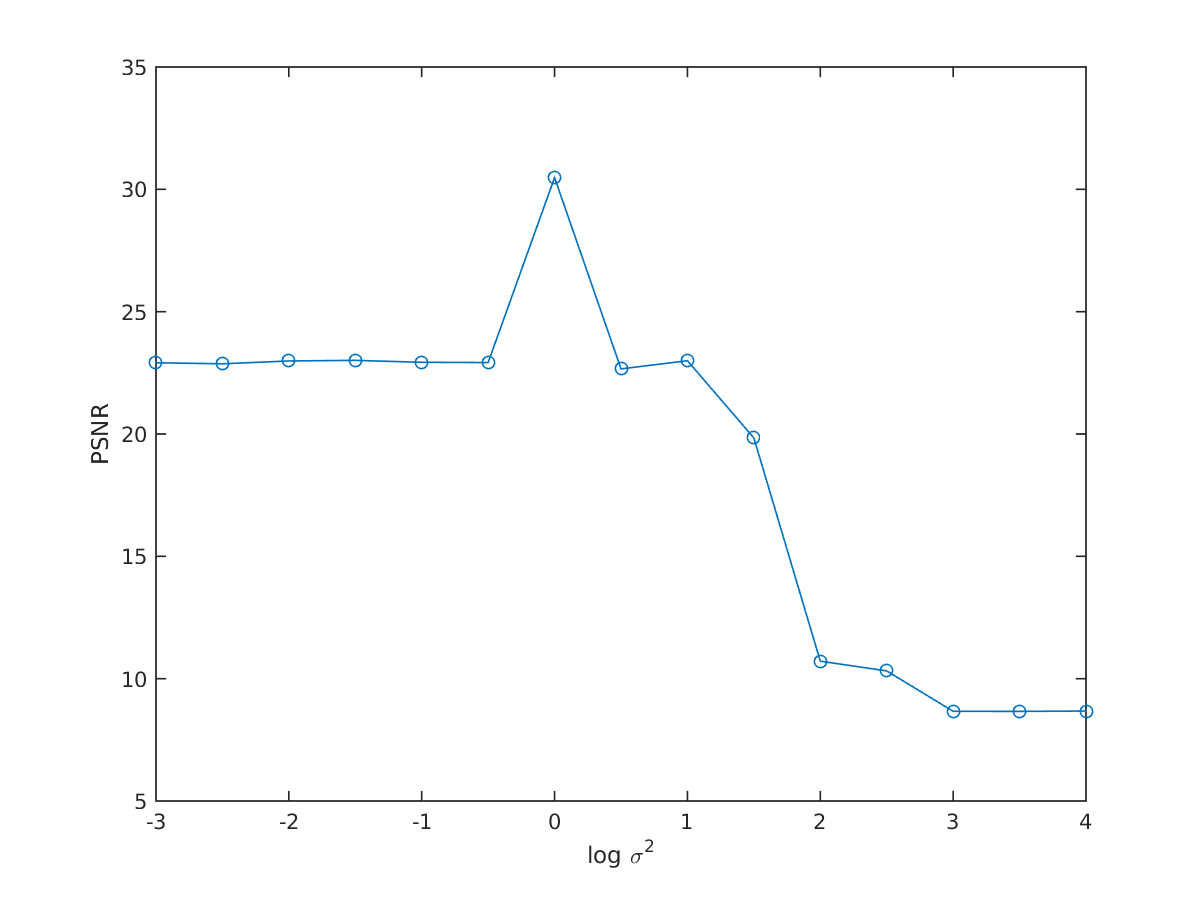
\includegraphics[width=\textwidth]{Chapter7/Images/noise_lenna_wide.png}
\end{figure}

% \begin{figure}
% \centering
% \begin{subfigure}{0.4\textwidth}
% 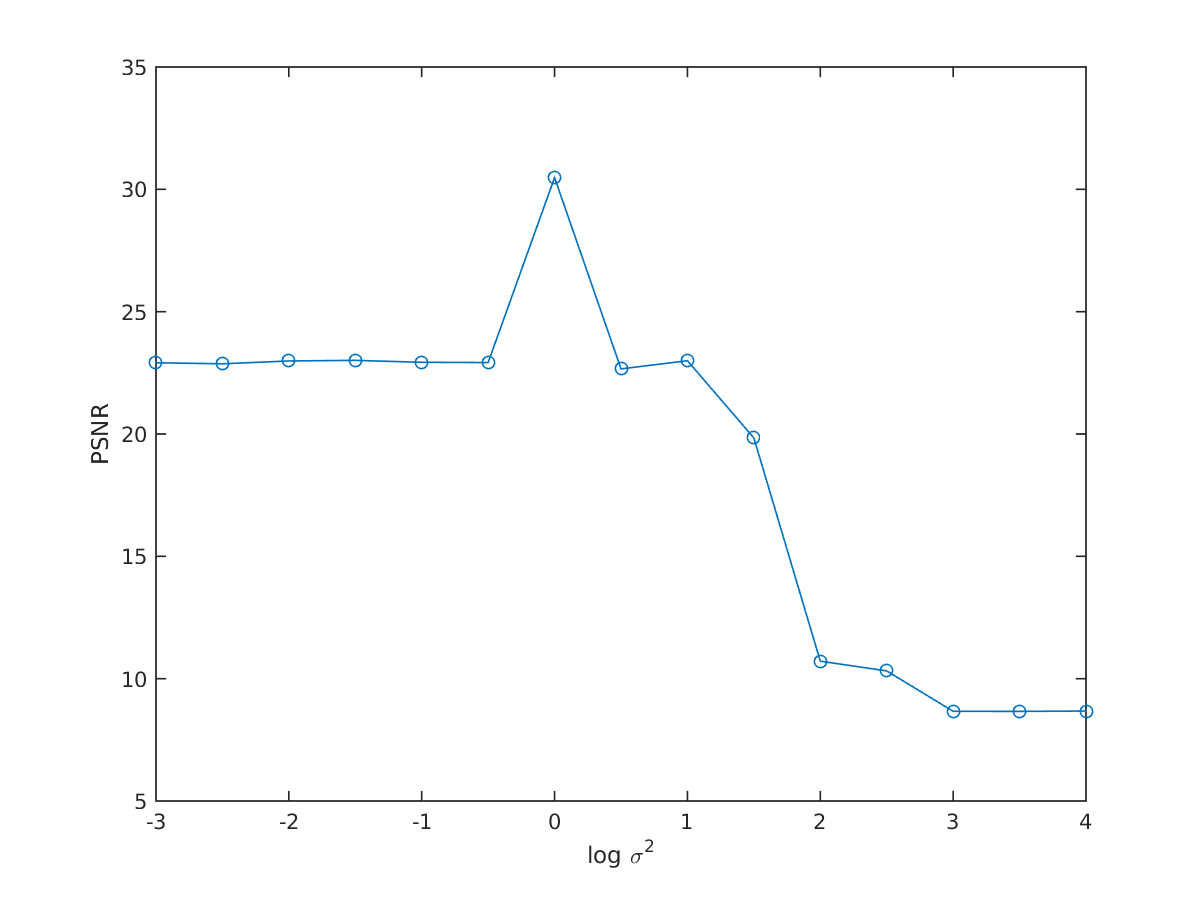
\includegraphics[width=\textwidth]{Chapter7/Images/noise_lenna_wide.png}
% \end{subfigure}
% \begin{subfigure}{0.4\textwidth}
% 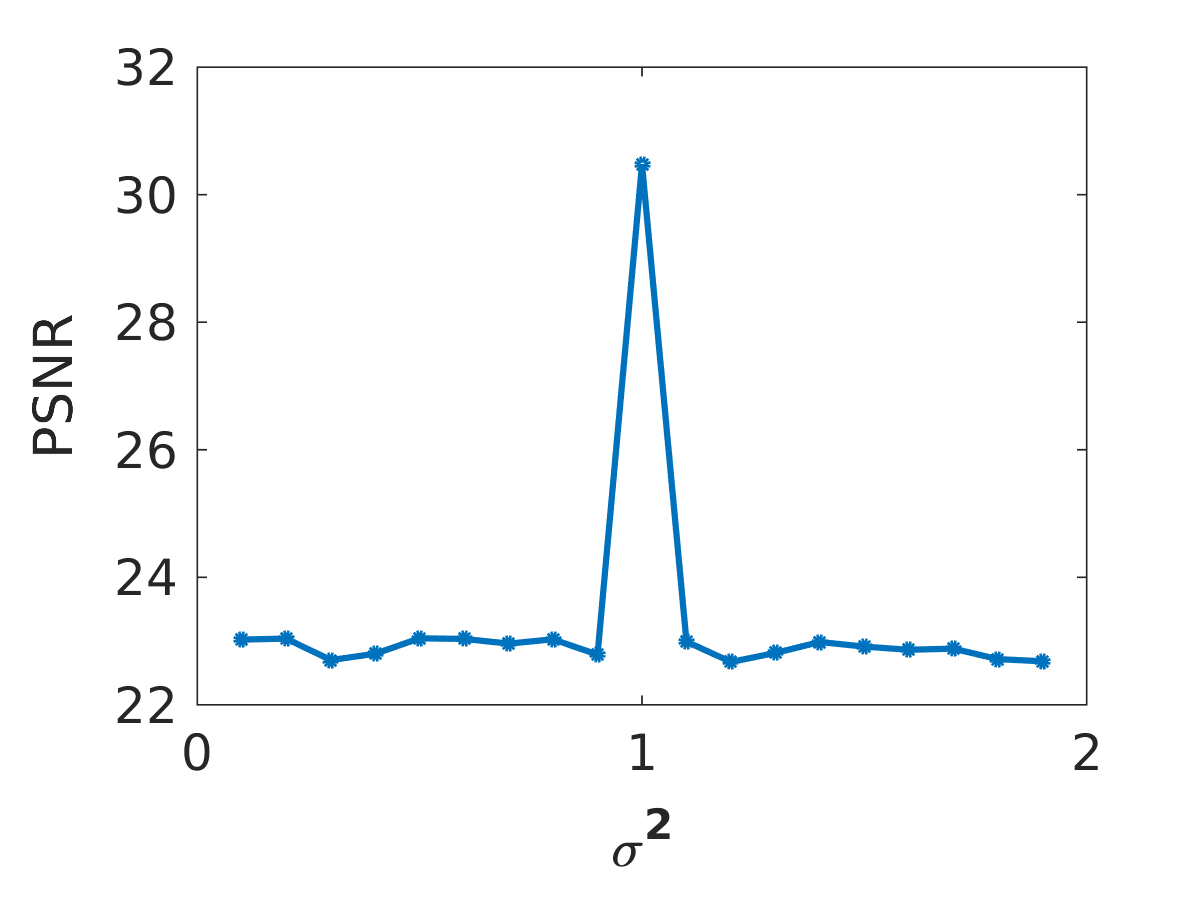
\includegraphics[width=\textwidth]{Chapter7/Images/noise_lenna_close.png}
% \end{subfigure}
% \begin{subfigure}{0.4\textwidth}
% 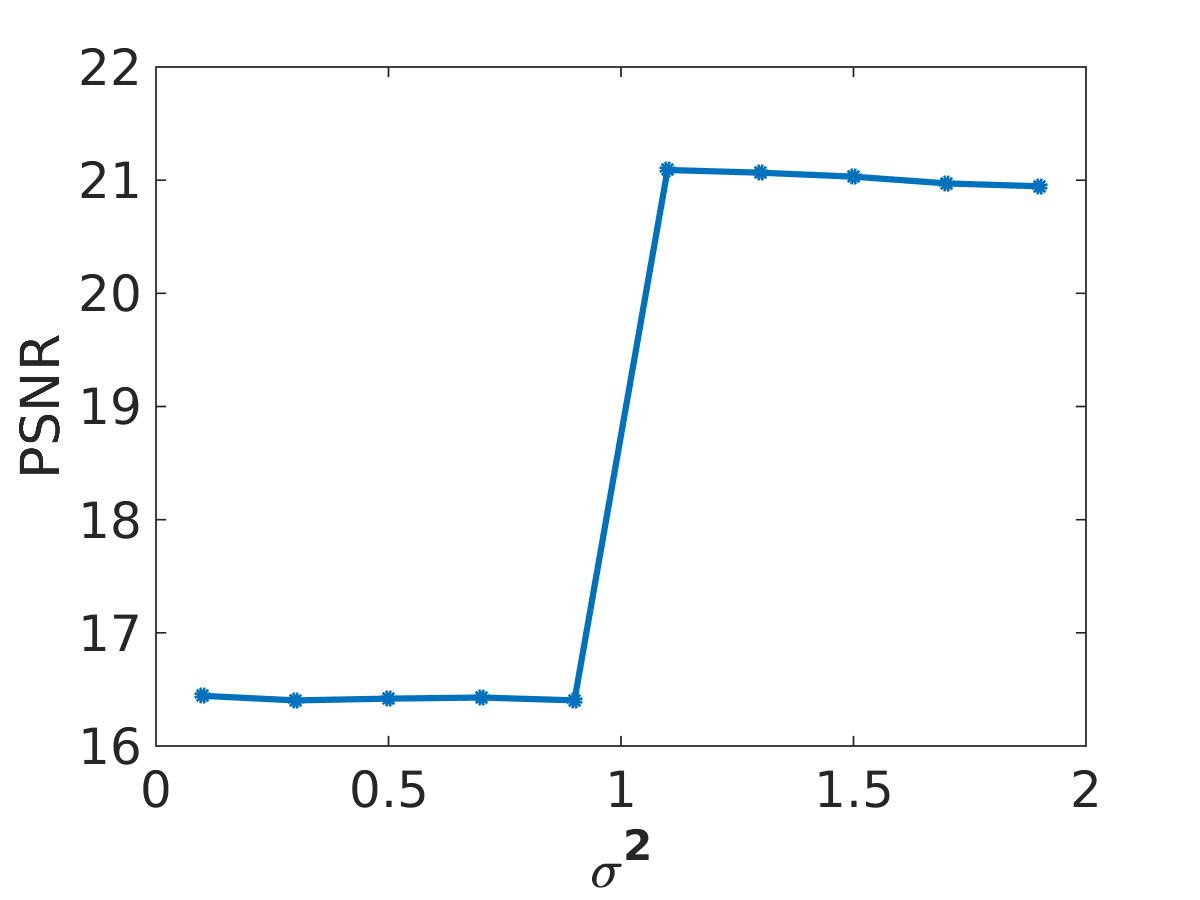
\includegraphics[width=\textwidth]{Chapter7/Images/noise_foreman_close.png}
% \end{subfigure}
% \begin{subfigure}{0.4\textwidth}
% 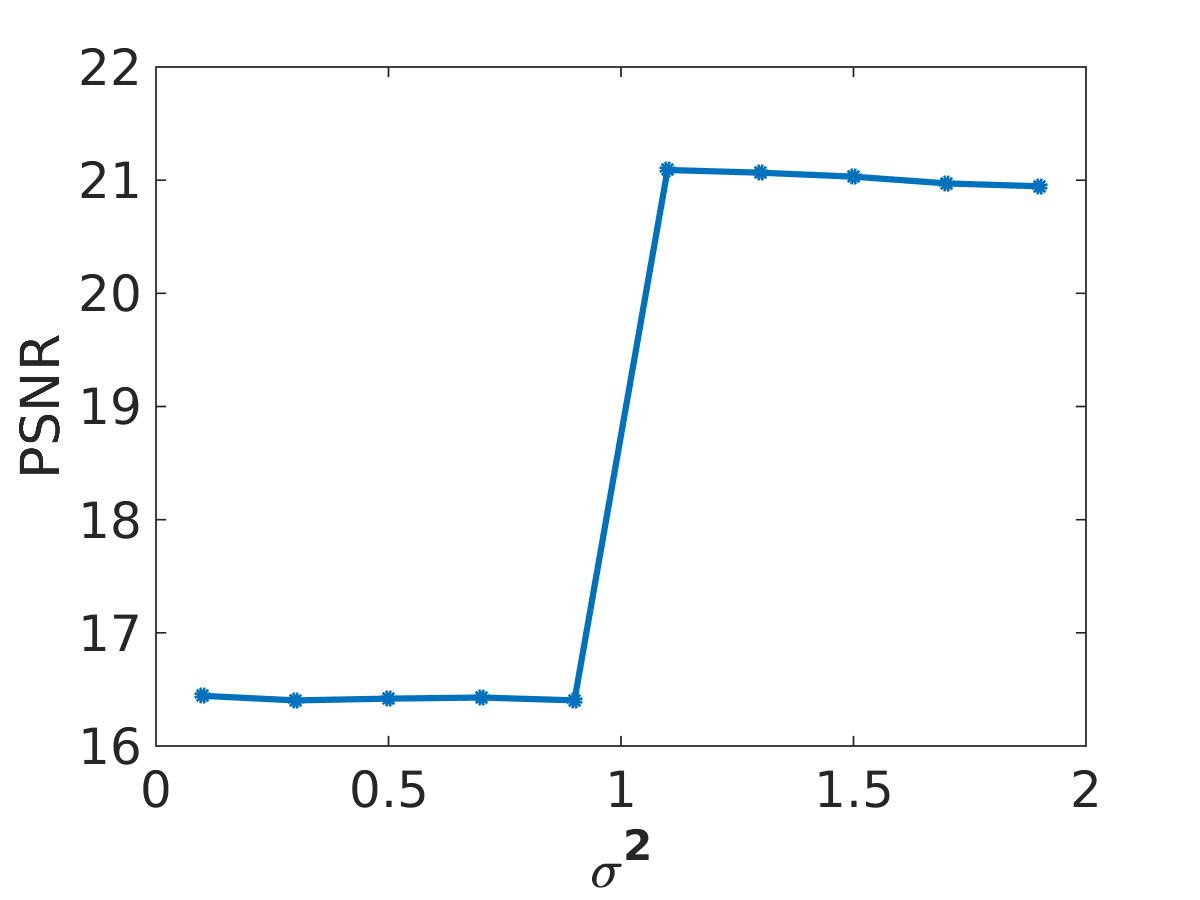
\includegraphics[width=\textwidth]{Chapter7/Images/noise_foreman_close.png}
% \end{subfigure}
% \end{figure}

\subsection{Noise Threshold \texorpdfstring{$\tau$}{[tau]}}

\section{Example Results}
Different Decimation Patters. 

Different Percentages. 

Different block size.

\section{Comparison of MSCE against BCS with DCT for interpolation}

Performance curve

What if pre-compressed

Comparison with literature?

\section{Analysis of Speed}
Time vs block dim.

Serial vs MPI.


\section{Video Reconstruction for General Sensing Matrices}

\begin{itemize}
\item General sensing Matrix for BCS of videos?
\item Masks vs Gaussian vs Rademacher
\item MSCE was done to solve the signal interpolation. In particular, to fix the problem with small support of wavelets while still using their power.
\item Problem: Limited to signal interpolation. Solution: Use CS sensing matrices (but Cascade don't work yet).
\end{itemize}
